% !TeX root = SA_Rockstroh_Main.tex
\chapter{Vorbetrachtung}
\label{Ch:Vorbetrachtung} 
% Vorwissen:
% - Grund des Kataloges
% - Prinzipielle Funktion/Nutzen
%
% =-- Vor dem Schreiben angedachter Inhalt ---=
%Inhalt:\\
%Grundgedanken zu Modellkatalog. Ansprüche. Wünsche bzgl. Funktionsumfang und Anwendbarkeit, Prinzip: aufwändiges Hinzufügen, einfaches Anwenden \\
%Ist-Stand: Was gibt es für vergleichbare Kataloge/Projekte? + Bewertung dieser\\
%Beschreibung der aktuellen Situation zur Modellfindung --> Zeitintensive suche nach Publikationen, nur ausgewählte Eigenschaften benannt und untersucht, teils uneinheitliche, unübersichtliche, komplexe Modelldarstellung, Reproduzierbarkeit der Implementierung der Ergebnisse einer Publikation aber auch allein schon des Modells oft sehr schwierig \\
%Grundüberlegungen zu den nützlichen Elementen des Kataloges: \\ Modell als Art Datenbankeintrag (Erschließbarkeit über Suche --> Einheitliche Attributsnamen (--> KS) + Bedeutung, Erweiterbarkeit), \\ Textuelle (semantische?) Modelldarstellung mit einheitlicher Struktur und Modellnotation, \\einheitliche Implementierung die einfache Nutzbarkeit der Modelle erlaubt \\
%Umsetzung der einzelnen Elemente: \\
%Metadata-File: Struktur aus ACKRep übernommen - leicht Angepasst \\
%Klassifikationssystem: Semantische, ontologische Ausarbeitung des auf Modelle anwendbaren Teilbereich der Regelungstheorie, Anforderungen explizit? --> Graphentheorie, Finden einer fachlich korrekten, eindeutigen - in Bezug auf Ontologie selbst und auf Anwendung auf Modelle - und verständlichen Darstellung (Beispiel Polynom --> linear/nicht-linear) und Namensgebung (strictly\_non\_linear)\\ 
%Textuelle Repräsentation: Struktur abgeleitet aus (guten) Publikationen[Referenzen], sinnvolle Informationsreihenfolge, Offenhaltung von Gestaltungsspielraum in Anbetracht des Umfangs der Regelungstechnik \\ 
% =-- Vor dem Schreiben angedachter Inhalt ---=
%
%Alternative Struktur: 	Section: Aktueller Stand (der Modellsuche und von Modellkatalogen)
%						Section: Prozess der Katalogerstellung/ Grund-/Vorgedanken zum Katalog
%						Subsections: Anforderungen - Kurze Diskussion was sinnvoll, Struktur, Elemente

%TODO: Neue Formulierung für Einstieg in Ch:1
Der in \ref{Ch:Ergebnisse} vorgestellte Katalog und dem dazugehörigen Klassifikationssystem ist das Resultat vieler Entscheidungen. Dem ist eine Recherche von Literatur mit regelungstechnischen Modellen voraus gegangen. Das Kapitel beginnt mit einer Erklärung zu den Begriffen \textit{System} und \textit{Modell}. Anschließend wird in \ref{Ch:Vorbetrachtung:Sec:CurrentState} der aktuelle Stand der Modellrecherche und vorhandener Modellsammlungen vorgestellt. Danach werden in \ref{Ch:Vorbetrachtung:Sec:Anforderungen} die Anforderungen für den Katalog formuliert und getroffene Entscheidungen vorgestellt, die zur Erfüllung der Anforderungen beitragen sollen. Bevor in \ref{Ch:Vorbetrachtung:Sec:KS} die wichtigsten Entscheidungen zur Erstellung des Klassifikationssystems vorgestellt werden, gibt es in \ref{Ch:Vorbetrachtung:Sec:Wissensrepräsentaionen} noch eine Einführung zu Wissensrepräsentationen und die Graphentheorie.   

% ===================================================================
% ------------- SECTION: Dynamische Systeme und Modelle -------------
% ===================================================================
\section{Dynamische Systeme und Modelle}
\label{Ch:Vorbetrachtung:Sec:SystemeModelle}
Die Begriffe \textit{System} und \textit{Modell} kommen in der regelungstechnischen Literatur häufig vor. Die Bedeutung kann, je nachdem in welchen Anwendungsgebiet diese verwendet werden, stark variieren. Und selbst innerhalb regelungstechnischer Literatur werden beide Begriffe eher selten extra definiert oder referenziert, sondern auf Basis eines intuitiven Verständnisses verwendet. Für diese Arbeit, die den Begriff \textit{Systemmodelle} schon im Titel trägt, sind beide Begriffe bedeutsam, weshalb an dieser Stelle beschrieben wird wie diese Begriffe in dieser Arbeit verstanden werden sollen.

Ein \textit{System} ist nach \textit{DIN IEC 60050-351:2014-09}\footnote{siehe \cite{DINIEC60050-351} Seite 21} eine \glqq Menge miteinander in Beziehung stehender Elemente, die in einem bestimmten Zusammenhang als Ganzes gesehen und als von ihrer Umgebung abgegrenzt betrachtet werden\grqq.\\
Des weiteren wird in den Anmerkungen der Norm ausgeführt, das die Elemente eines Systems \glqq natürliche oder künstliche Gegenstände sowie Arten von Denkvorgängen und deren Ergebnisse\grqq sein können und dass das System \glqq von der Umgebung und von den anderen äußeren Systemen durch eine gedachte Hüllfläche abgegrenzt betrachtet\grqq wird.

Ein System wird in dieser Arbeit als \textit{reales System} bezeichnet, wenn dessen Element nachweisbare Bestandteile der Realität sind.

\textit{Modelle} sind (nach Stachowiak\cite{STA73} S. 131ff) Abbildungen oder Repräsentationen natürlicher oder künstlicher Originale, welche selbst wieder Modelle sein können(\textit{Abbildungsmerkmal}). Zudem haben Modelle immer nur eine Auswahl der Attribute des Originals, welche dem Modellersteller und/oder dem Modellnutzer als relevant erscheinen(\textit{Verkürzungsmerkmal}) und Modelle dienen einem bestimmten Zweck(\textit{pragmatisches Merkmal}). 

Ein System oder Modell ist \textit{dynamisch}, wenn sich dessen Werte mit der Zeit verändern. Die Regelungstechnik beschäftigt sich unter anderem damit das zeitveränderliche Verhalten von Systemen und Modellen zu untersuchen und zu beeinflussen. Deshalb sind für diese Arbeit nur dynamische Systeme und Modelle von Interesse und die Begriffe \textit{System} und \textit{Modell} implizieren in dieser Arbeit die Eigenschaft \textit{dynamisch}. 

Modelle von Systemen(\textit{Systemmodelle}) bestehen in der Regelungstechnik zum einen aus einer graphischen Repräsentation des Systems, die wiederum aus definierten Formen besteht welche die Elemente des Systems repräsentieren und zum anderen aus einem mathematischen Modell, welches das Verhalten des Systemmodells beschreibt. Ein System kann mehrere Modelle in Form einer graphischen Repräsentation haben, wobei es zu jedem Modell wiederum verschiedene mathematische Modelle geben kann(vgl. \cite{LUD95} Sektion 2.1).\\
Ein \textit{mathematisches Modell} ist ein Modell das die Anwendung mathematischer Methoden erlaubt(\cite{GRVO16}, S.9). Das mathematische Modell ist in der Regelungstechnik üblicherweise ein System von Gleichungen. 

% BILD: System --> Modelle --> Math. Modelle
% ==========================================
\begin{figure}[H]
	\centering
	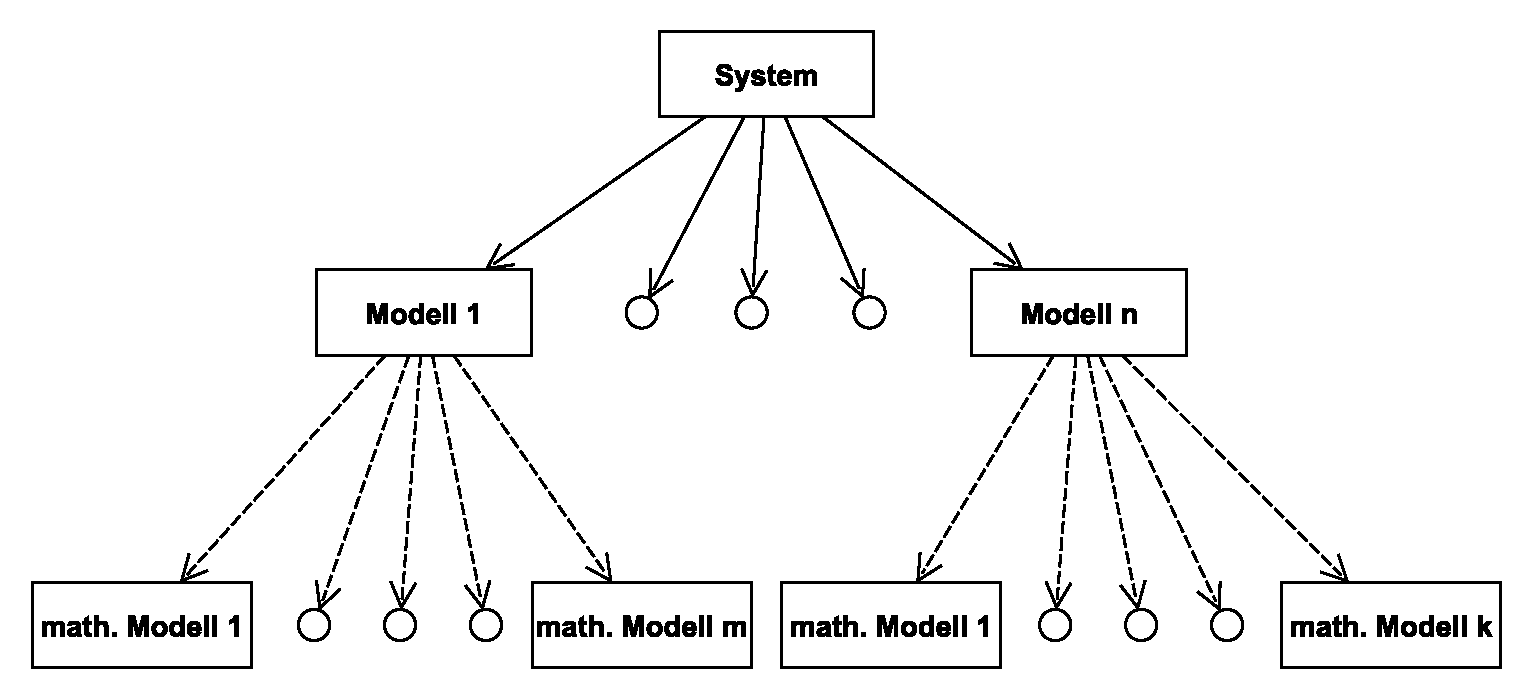
\includegraphics[width=0.9\linewidth]{Systeme_Modelle_Math_Beschreibung}
	\caption{Zusammenhang Systeme, Modelle und mathematische Modelle}
	\label{fig:SysModelleSkizze}
\end{figure}

Zudem gibt es in der Regelungstechnik Modelle, die ausschließlich aus dem mathematischen Modell, also einer Beschreibung des dynamischen Verhaltens, bestehen. Diese Modelle repräsentieren kein Original und werden in dieser Arbeit als \textit{abstrakte Modelle} bezeichnet. Abstrakte Modelle lassen sich in den obigen Modellbegriff integrieren, indem gesagt wird das für jedes abstrakte Modell ein System gedacht werden kann, welches nicht bekannt ist. 

Der Begriff \textit{System} bezeichnet im Folgenden dynamische Systeme. Der Begriff \textit{Modell} bezeichnet im Folgenden sowohl dynamische Systemmodelle als auch dynamische abstrakte Modelle.
% Ein Beispiel für ein System wäre ein realer elektrischer Schaltkreis der durch ein elektrisches Netzwerk modelliert wird. Ein elektrisches Netzwerk enthält z.\,B. Induktivitäten und Kapazitäten, welche reale Entitäten wie % Spulen und Kondensatoren repräsentieren.

% ====================================================
% ------------- SECTION: Aktueller Stand -------------
% ====================================================
\section{Aktueller Stand}
\label{Ch:Vorbetrachtung:Sec:CurrentState}
Für die Suche nach Modellen und Modelleigenschaften war viel Recherche notwendig, welche zu den in diesem Abschnitt beschriebenen Erkenntnisse bezüglich der Modellfindung geführt hat.
% ============================================================
% ------------- Aktuelle Situation Modellfindung -------------
% ============================================================
\textbf{Aktuelle Situation der Modellfindung}: 
% Auflistung von aufgefallenen Aspekten + Beispielhafte Nennung von Publikationen  
\begin{enumerate}
	\item Regelungstechnische Modelle finden sich aktuell meist verteilt in wissenschaftlichen Publikationen, wie z.B. Lehrbüchern, Artikeln, Dissertationen, Diplom- und Studienarbeiten.
	\item Die Qualität der Modelldarstellung ist uneinheitlich. Das die Modellgleichungen eindeutig gekennzeichneten und gemeinsam notiert, sowie die eingeführten Variablen gut beschrieben und klar definierten Typs (Parameter, Eingangs-, Zustandsvariable) sind ist nicht immer gegeben.
	\begin{itemize}[label=$\bullet$]
		\item Beispiel 1: In \cite{LOR63} wird auf Seite 135 das Modell eines dynamischen Systems übersichtlich dargestellt. Es ist abhängig von den Parametern $\sigma$, $r$ und $b$. Die Zustandsvariablen und der Parameter $\sigma$ werden direkt nach den Modellgleichungen beschrieben. Die Parameter $r$ und $b$ haben hingegen keinen Namen und werden nur als Gleichungen repräsentiert. Der Parameter $b$ hängt wiederum von $a$ ab, welches in dem Artikel auch nicht explizit eingeführt wird.
		\item Beispiel 2: In \cite{YIFREA09} wird eine Walzstrecke für Metalle modelliert. Die Variablen werden am Anfang alle eingeführt und danach wird das Modell ausführlich hergeleitet. Eine zusammengestellte Übersicht der Modellgleichungen fehlt jedoch. Die Zustandsvariablen müssen aus Ausgangsvektor und Abbildungen erschlossen werden. Die Modellgleichungen sind im Artikel verteilt.
	\end{itemize}
	\item Die mathematische Darstellungsform der Modellgleichungen kann sich unterscheiden.
	\begin{itemize}[label=$\bullet$]
		\item Beispiel 3: In \cite{SILEEA12} Seite 14 werden die Gleichungen des Modells als Gleichungssystem von gewöhnlichen Differentialgleichungen(DGLn) erster Ordnung dargestellt. Die Gleichungen sind jedoch nicht wie üblich umgestellt\footnote{Üblicherweise werden die Modellgleichungen so umgestellt, das sich die Zeitableitungen der Zustände möglichst allein auf der linken Seite und das sich die restlichen Variablen und nicht-abgeleiteten Zustände auf der rechten Seite der Gleichung befinden.}, denn auf der linken Seite der Gleichungen befinden sich Summen aus Zeitableitungen und nicht-abgeleiteten Zustandsgrößen.
		\item Beispiel 4: In \cite{BUT21} Seite 3 besteht das mathematische Modell des Systems aus einer gewöhnlichen DGL zweiter Ordnung
		\item Beispiel 5: In \cite{KNO16} Seite 168f, Beispiel B.3 besteht das mathematische Modell des betrachteten Systems aus einem gewöhnlichen Differentialgleichungssystem zweiter Ordnung, wobei wie in Bsp. 3 diese nicht wie üblich umgestellt worden sind.
	\end{itemize}
	\item  Die Modelleigenschaften sind oft nur implizit gegeben, z.B. kann bei einem Steuerungsentwurf geschlussfolgert werden, dass das untersuchte System stabil ist. Die explizite Nennung von Modelleigenschaften erfolgt meist nur, wenn diese für die Publikation von Relevanz sind. 
	\begin{itemize}[label=$\bullet$]
		\item Beispiel 6: Im Artikel \cite{PEGUEA16} Seite 761, letzter Abschnitt wird auf die Steuerbarkeit der Modelldarstellung eingegangen. Andere Eigenschaften finden keine Erwähnung.
	\end{itemize}
	\item In nahezu allen Publikationen erfolgt die Erprobung der Ergebnisse mittels Simulation. 
	\begin{itemize}[label=$\bullet$]
		\item Beispiel 7: In \cite{BUT21} wird der Verlauf der Eingangswerte, welcher für die im Dokument gezeigten Simulationsergebnisse verwendet wurde, nur als grauer Graph gezeigt. Eine Angabe der Gleichung für die Eingangswerte fehlt. Ebenso wird z.\,B. der verwendete Parameterwert für die Gleichspannung $v_DC$ nicht gegeben.
	\end{itemize}
	\item Die genutzte Implementation wird nicht publiziert bzw. veröffentlicht.
\end{enumerate}

% Schlussfolgerung aus den aufgefallenen Aspekten
\textbf{Feststellung}:\\
Die zielgerichtete Suche nach Modellen, z.\,B. mit bestimmten Eigenschaften, ist oft eine zeitintensive und aufwendige Angelegenheit. Zudem braucht es häufig zusätzliche Eigenarbeit um zu einer brauchbaren Modelldarstellung zu gelangen. Die Implementierung muss aktuell fast immer von eigener Hand erfolgen. Für die Validierung des eigenen Codes und die Reproduktion der Resultate einer Publikation ist oft eine softwaretechnische Implementation des Modells sowie der daran angehängten Umgebung (Steuerung, Regelung, Beobachter etc.) notwendig (vgl. \cite{KNHE20b}, Seite 1). Durch eben Aspekte ist das meist aufwendig oder nicht möglich.

% ===============================================================
% ------------- Aktuelle Situation Modellsammlungen -------------
% ===============================================================
\textbf{Aktuelle Situation von Modellsammlungen und -katalogen}: \\
Bestehende Zusammenstellungen von regelungstechnischen Modellen sind schwer zu finden. Ein Grund dafür könnten sein, das wenige existieren. Es könnte aber auch daran liegen, das diese einfach nur schwer zu finden sind. Zum Beispiel, weil diese z.\,B. von der Suchmaschine als nicht relevant eingestuft werden und dementsprechend auf den hinteren Seiten der Suchergebnisse landen. Zudem basieren die Suchergebnisse nur auf den eingegebenen Wörtern. Ein Verständnis für den Kontext fehlt, was zu einer großen Anzahl an Suchergebnissen führt. Es ist also durchaus plausibel das mehr als die jetzt aufgeführten Zusammenstellungen existieren. 

\textbf{The Automatic Control Knowledge Repository (ACKRep)}:\\
Das in \cite{KNHE20a} vorgestellte ACKRep\footnote{ACKRep Testinstanz. \tiny{URL}\normalsize: \url{https://testing.ackrep.org/}} ist ein Tool, mit dem Ziel die implementierten Ergebnisse von Publikationen reproduzierbarer zu machen. Es besteht aus einer Datenbank von implementierten Problemspezifikationen, Lösungsmethoden und Softwareumgebungen, die in ihrem Zusammenwirken die Ergebnisse reproduzierbar machen sollen. Die Einträge vom Typ \textit{ProblemSpecification} enthalten dabei Modelle, die als Python-Quellcode repräsentiert werden bzw. implementiert sind. Weitere Informationen zu den Modellen wie der Identifikationsschlüssel, externe Referenzen und Modelleigenschaften sind in einer Metadaten-Datei im YAML-Format hinterlegt. Für die einheitliche Benennung der Modelleigenschaften wird auf die in \cite{KNHE20b} eingeführte \textit{Ontology of Control Systems Engineering (OCSE)}\footnote{Die \textit{OCSE} ist eine Wissensrepräsentation(siehe \autoref{Ch:Vorbetrachtung:Sec:Wissensrepräsentaionen}) zur Regelungs- und Steuerungstheorie.} zurück gegriffen.

\textbf{Beispiele unteraktuierter mechanischer Systeme in \cite{LIYU13}}:\\
Im Zuge der Betrachtung unteraktuierter mechanischer Systeme werden in dem Artikel die Modellgleichungen von 11 Beispielen tabellarisch in einer vereinheitlichten Form aufgeführt, deren mathematisches Modell aus gewöhnlichen DGLn zweiter Ordnung besteht. Zudem werden die Systeme bezüglich ihrer Beschränkungen, ihrer Konfigurationscharakteristik und ihrer regelungstechnischen Problemstellung klassifiziert.

% Vergleich der beiden Beispiele
Die beiden Zusammenstellungen haben einen unterschiedlichen Fokus.\\
Im ACKRep liegt der Fokus auf der Implementierung der Modelle. Ein weiterer Fokus liegt auf der Auffindbarkeit der Modelle innerhalb des ACKReps. Dafür ist eine Suchfunktion angedacht, die eine gefilterte Ausgabe der Elemente ermöglichen soll.\\
In \cite{LIYU13} liegt der Fokus auf der menschlichen Lesbarkeit. Die Modellgleichungen sind als Text bzw. Formeln repräsentiert und ermöglichen die Anwendung von analytischen Methoden. 

Beide Zusammenstellungen haben gemeinsame, dass eine einheitliche Form für die Modellrepräsentation verwendet wird. Zudem findet bei beiden eine Klassifikation statt, welche sich allerdings in Umfang und Inhalt unterscheiden.
\section{Anforderungen an den Katalog} % Alternativer Titel: Prozess der Katalogerstellung
\label{Ch:Vorbetrachtung:Sec:Anforderungen}
\textbf{Anforderungen an den Katalog}:\\ %Vielleicht als Enumeration schreiben?
% =========================================
% ------------- Anforderungen -------------
% =========================================
Der Katalog soll den Prozess der Modellfindung und Nutzung vereinfachen, sodass die in \autoref{Ch:Vorbetrachtung:Sec:CurrentState} beschriebenen Schwierigkeiten nicht durchlaufen werden müssen. Daher wurden für den Katalog folgende Anforderungen formuliert.
\begin{enumerate}[label=\textbf{Anforderung A.\arabic*}:, ref=\textbf{A.\arabic*}, wide=0pt, leftmargin=*]
	\item \label{A.Findbarkeit}Neue Modelle sollen einfach und unkompliziert zu finden sein.
	\item \label{A.Modelleigenschaften}Die Modelleigenschaften sollen so gut wie möglich erfasst sein. Das heißt:
	\begin{itemize}[label=$\bullet$]
		\item Sie sollen möglichst vollständig sein.
		\item Sie sollen eine übersichtliche Darstellungsform haben.
		\item Sie sollen einer einheitlichen Namensgebung folgen.
		\item Sie sollen eine Definition haben.
	\end{itemize}
	\item \label{A.Darstellung_Gleichungen}Die Modelle sollen eine einheitliche Darstellungsform haben.
	\item \label{A.Darstellung_Variablen}Die Variablen, deren Typ und Bedeutung sollen in einer sinnvollen, einheitlichen Darstellung notiert sein.
	\item \label{A.Implementierung}Die Modelle sollen möglichst implementiert vorliegen. Die Implementierung soll einfach verwendbar sein.
	\item \label{A.Erweiterbarkeit}Der Katalog soll erweiterbar sein. % durch externe Personen/Nutzer
\end{enumerate}

% ==========================================
% ------------- Entscheidungen -------------
% ==========================================
Die Anforderung \ref{A.Erweiterbarkeit} macht es notwendig den Fall einer zukünftig großen Anzahl im Katalog existierender Modelle mitzudenken. Mit zunehmender Modellanzahl wird es aufgrund abnehmender Übersichtlichkeit schwieriger bestimmte Modelle im Katalog zu finden. Dazu kommt, das es auch wünschenswert ist nach Modellen suchen zu können, die bestimmte Kriterien erfüllen. Das macht eine Suchfunktion erstrebenswert um die Anforderung \ref{A.Findbarkeit} zu erfüllen. Um eine Suchfunktion zu realisieren wird eine Datenbank benötigt, die überhaupt erst mal durchsucht werden kann. Die Erstellung einer Suchfunktion und der dafür benötigten Datenbank soll durch folgende Entscheidung erleichtert werden:
\begin{enumerate}[label=\textbf{Entscheidung E.\arabic*}:, ref=\textbf{E.\arabic*}, wide=0pt, leftmargin=*]
	\item \label{E.MetadatenDatei}Zu jedem Modell soll eine Datei \textit{(Metadaten-Datei)} geben, in der wichtige Informationen wie der Modellschlüssel und -Name, die Modelleigenschaften und der Modellersteller hinterlegt werden. Die Metadaten-Datei soll im einfach les- und editierbaren YAML Format vorliegen.
\end{enumerate}
Die Idee und Umsetzung von Entscheidung \ref{E.MetadatenDatei} basiert auf \cite{KNHE20a}. Die Struktur der Metadaten-Datei wurde aus dem \textit{ACKRep} übernommen und leicht angepasst.

Anforderung \ref{A.Modelleigenschaften} soll durch das in der Aufgabenstellung geforderte \textit{Klassifikationssystems (KS)}(siehe \autoref{Ch:Vorbetrachtung:Sec:KS} und \autoref{Ch:Ergebnisse:Sec:KS}) und die Anwendung dessen auf die Modelle erfüllt werden. Die Auflistung der Modelleigenschaften eines Modells erfolgt in der Metadaten-Datei. Die Verwendung der im KS verwendeten Namen für die Modelleigenschaften sorgt für eine einheitliche Namensgebung. Die Definition der Modelleigenschaften und der Beziehungen zwischen diesen basieren auf im KS enthaltenen Referenzen. Die folgende Entscheidung befasst sich mit der technischen Umsetzung des KS.
\begin{enumerate}[resume*]
	\item \label{E.KS_TechUmsetzung}Die Einträge des KS werden im YAML Format gespeichert. Um eine grafische Darstellung des KS zu erhalten soll ein Python-Skript geschrieben werden, welches diese als Bilddatei des KS erstellt.
\end{enumerate}
Wie vollständig die in der Metadaten-Datei enthaltenen Modelleigenschaften sind hängt davon ab, wie gut erforscht das Modell ist\footnote{Damit ist gemeint, das es einfach noch nicht bekannt ist, ob ein Modell bestimmte Eigenschaften hat oder nicht.} und wie viel Zeit in das Anlegen des Modells gesteckt wird.

In Textform dargestellt Modelle haben den Vorteil das in Formeln verwendete Elemente wie Tiefsetzungen und Brüche grafisch dargestellt werden können. Im Fließtext muss die Umsetzung der Elemente über ein Notationssytem erreicht werden, welches die Lesbarkeit verringert ($1/3$ statt $\frac{1}{3}$ oder $F\_1$ statt $F_1$). Eine für Menschen gut lesbare Notation der Modellgleichungen macht die Arbeit mit diesen einfacher und ist generell erstrebenswert, weshalb folgende Entscheidung getroffen wurde. 
\begin{enumerate}[resume*]
	\item \label{E.Textdok}Die Modellgleichungen und die zugehörigen Variablen werden in Textform notiert. Grundlage ist ein \LaTeX-Dokument, das in eine PDF-Datei umgewandelt wird. Die Modellgleichungen werden als System von Differentialgleichungen erster Ordnung dargestellt. Die Auflistung der Variablen und ihrer Bedeutung erfolgt gebündelt.
\end{enumerate}
Die Bündelung der Variablendefinitionen innerhalb der Textrepräsentation macht diese gut im Dokument auffindbar und erfüllt Anforderung \ref{A.Darstellung_Variablen}. Die Festlegung auf die Verwendung von DGLn erster Ordnung ist zum einen recht allgemeingültig, da DGLn höherer Ordnung durch Einführung definitorischer Gleichungen in ein System von DGLn erster Ordnung überführt werden können, und zum anderen die in Publikationen am häufigsten verwendete Form der Darstellung der Modellgleichungen. Zudem wird durch diese Festlegung die Anforderung \ref{A.Darstellung_Gleichungen} erfüllt.

Anforderung \ref{A.Implementierung} fordert die Implementierung der Modelle. Darauf bezieht sich die nächste Entscheidung.
\begin{enumerate}[resume*]
	\item \label{E.Implementation}Die Modelle werden in der Programmiersprache Python implementiert. Dabei soll jedes Modell als Python-Klasse umgesetzt werden.
\end{enumerate}
Die Implementierung der Modelle als Klasse soll den zweiten Teil von Anforderung \ref{A.Implementierung} erfüllen. Die Modelle werden in der Verwendung als Objekt der Modellklasse instanziiert, was für das Verständnis eine einfache und intuitive Analogie zur realen Welt ist in der reale Systeme als physische Objekte existieren. Die Modellklasse ist in dieser Analogie der Bauplan und das instanziierte Objekt ein spezifischer Aufbau des Systems. Zudem können innerhalb des instanziierten Objektes eine Reihe von Informationen zu dem spezifisch implementierten Modell gespeichert werden. Die Verwendung für eigene Simulationen ist damit sehr unkompliziert, da nur noch der Code für die Simulationsparameter sowie die Aufzeichnung und grafische Darstellung der Simulationsergebnisse selbst geschrieben werden muss. Die für die Simulation benötigten Modellgleichungen können über die Methoden der Klasse direkt verwendet werden.

Es stellte sich noch die Frage, ob alle Modelle des Kataloges implementiert vorliegen müssen. Denn zum Einen ist die in Anforderung \ref{A.Darstellung_Gleichungen} geforderte einheitliche Darstellung der Modellgleichungen an sich schon durch die in Entscheidung \ref{E.Textdok} beschriebene Textform gegeben. Zum Anderen sind einige Modelle recht schwer zu implementieren, wie z.\,B. Modelle deren Verhalten durch partiellen Differentialgleichungen beschrieben werden. Um eine hohe Modellvielfalt für den Katalog zu ermöglichen, wurde die folgende Entscheidung getroffen.
\begin{enumerate}[resume*]
	\item \label{E.ImplementierungOptional}Die Implementierung eines Modells ist optional.
\end{enumerate}

Um die Verwendbarkeit der vorliegenden Modelle weiter zu vereinfachen erschien es sinnvoll ein Beispielset der Parameterwerte zur Verfügung zu stellen. Die Beispielwerte sollen in der Textform und in der Implementation vorliegen.
\begin{enumerate}[resume*]
	\item \label{E.Parameterwerte}Zu jedem Modell soll es ein Beispielset an Parameterwerte geben. Diese sollen sowohl in der Textform als auch in der implementierten Form stets identisch sein. Dafür sollen die Beispielwerte an einer zentralen Stelle notiert sein, von der Textform und Implementation die Werte beziehen.
\end{enumerate}

%TODO: z.B. Strukutr Formulierung fixen oder kick
Die Entscheidungen \ref{E.Textdok} und \ref{E.Implementation} haben als Folge, das für eine Erweiterung des Kataloges eine Einarbeitung in die Form der Implementation und der Textrepräsentation erfolgen muss. Die folgende Entscheidung soll die Einarbeitung für neue Nutzer aber auch generell das Erstellen von neuen Modellen vereinfachen. Außerdem soll diese zur konstanten Erfüllung der Anforderungen \ref{A.Darstellung_Gleichungen} und \ref{A.Darstellung_Variablen} bei Erweiterung des Kataloges durch neue Personen beitragen.
\begin{enumerate}[resume*]
	\item \label{E.Vorlagen}Für Implementation und Textrepräsentation sollen Vorlagen erstellt werden, welche die repetitiven Elemente, wie z.\,B. die Struktur, dieser enthält. 
\end{enumerate}

Für die Anforderungen \ref{A.Findbarkeit} und \ref{A.Erweiterbarkeit} ist es wichtig einen einfachen Zugang zu den Daten des Kataloges zu schaffen, denn zum einen werden für die individuelle Nutzung der Modelle die Dokumentation und Implementation als lokale Daten benötigt und zum anderen müssen die Vorlagen lokal vorliegen um neue Modelle anlegen zu können.
\begin{enumerate}[resume*]
	\item \label{E.Git}Der Katalog soll als ein Git-Repositorium angelegt werden.
\end{enumerate}
Git ist eine dezentrale Versionsverwaltungssoftware, die sich für die Arbeit an textbasierten Dateistrukturen bewährt hat. Ein Git-Repositorium(\textit{Git-Repo}) ist eine Menge von versionsverwalteter Informationen und ist üblicherweise ein Dateisystem bestehend aus Ordnern und Dateien. Ein Git-Repo kann als lokale Kopie heruntergeladen und lokal editiert werden. Die lokal vorgenommenen Änderungen eines Git-Repos können auf das originale oder offizielle Git-Repo übertragen werden. Das geschieht mittels einer Anfrage zur Übertragung der Änderungen(\textit{Pull-Request}), welche von den Inhabern des offiziellen Repos geprüft wird. Wird eine Pull-Request angenommen, so werden die im lokalen Repo vorgenommenen Änderungen auf das offizielle Repo übertragen(vgl. \cite{KNHE20a} Abschnitt 2.1).

Die folgenden Abschnitte behandeln den Prozess um das Wissen über Modelle und deren Modelleigenschaften formal darzustellen.
% ===================================================
% ------------- Wissensrepräsentationen -------------
% ===================================================
\section{Wissensrepräsentationen}
\label{Ch:Vorbetrachtung:Sec:Wissensrepräsentaionen}
Wissensrepräsentationen sollen das existierende Wissen innerhalb eines Wissensbereichs formal abbilden. Für die Bestandteile der Repräsentation wird ein explizites Vokabular genutzt und die Beziehungen zwischen den Bestandteilen werden definiert (vgl. \cite{BEN16} S.60, \cite{SEB04} S.1). Eine häufig verwendete Möglichkeit um eine formale Darstellung von Wissensrepräsentationen zu erhalten ist die Verwendung von Methoden und Begriffen aus der Graphentheorie.

Exkurs: \textit{Graphentheorie}\footnote{siehe \cite{STU09} S.29 und \cite{DIE20} Abschnitte 1.1, 1.3 und 1.10}\\
Ein \textit{Graph} besteht aus einer Menge von \textit{Knoten} $N$ und \textit{Kanten} $E$. Die Kanten verbinden die Knoten. Die Menge $E$ besteht also aus 2-Element Untermengen von $N$. Ein Element aus $E$ enthält also zwei Knoten, die durch eine Kante verbunden werden. Ist der Graph \textit{gerichtet}, so hat der Graph die zwei Funktionen $s:E\rightarrow N$ und $t:E\rightarrow N$ die jeder Kante $e$ einen Ursprungsknoten $s(e)$ und einen Endknoten $t(e)$ zuweisen. Kann der Graph mehrere Kanten zwischen denselben zwei Knoten haben, dann wird dieser \textit{gerichteter Multi-Graph} genannt. Zusätzlich kann die Menge $L$ und die Funktion $l$ eingeführt werden. Die Menge $L$ umfasst die Namen der Knoten und Kanten. Die Funktion $l:N\cup E\rightarrow L$ weißt jedem Knoten $n$ und jeder Kante $e$ einen Namen aus der Menge $l$ zu.
Ein gerichteter \textit{Pfad} ist ein Graph $P = (N, E)$, der zwei Knoten $x_1$ und $x_i$ eines Graphen $G$ über eine Sequenz von Kanten ($e_1$, $\dots$, $e_i$) verbindet. Ein Knoten kann maximal ein Mal entlang eines Pfades vorkommen. 
Zwei erwähnenswerte Spezialfälle von Graphen sind Bäume und kreisfreie Graphen. Ein Baum liegt vor, wenn jeder Knoten $n \epsilon N$ genau einen Nachfolger besitzen.\glqq Ein Graph heißt kreisfrei, wenn es keinen Knoten gibt der einen Pfad zu sich selbst hat. Kreisfreie gerichtete Graphen werden auch DAG(engl. \textbf{D}irected \textbf{A}cyclic \textbf{G}raph) genannt\grqq\footcite{STU09}. 

In Wissensrepräsentationen, die sich der Graphentheorie bedienen, steht jeder Knoten für einen Bestandteil der Repräsentation und jede Kante stellt eine Beziehung zwischen zwei Bestandteilen dar. Der Name der Kante definiert die Art der Beziehung. Für die Wissensrepräsentation gibt es verschiedene Formen die sich in ihrer semantischen Vielfalt unterscheiden. Beispiele solcher Formen sind: Taxonomie, Thesaurus, Semantisches Netz.\\ %TODO: Ontologie erwähnen?
Auf die Taxonomie und das Semantische Netz wird im Folgenden kurz eingegangen.
 
Die \textit{Taxonomie} ist eine der einfachsten Formen der Wissensrepräsentationen. Die Bestandteile dieser sind Kategorien die in eine Hierarchie aus Ober- und Unterkategorien gesetzt werden. Jede Kante stellt eine \glqq ist auch \grqq Beziehung dar. Jede Unterkategorie ist auch ein Element ihrer Oberkategorie. Die Darstellung kann über einen DAG erfolgen.

\textit{Semantische Netze} \glqq sind Graphen die Begriffe und ihre Relationen zueinander darstellen\grqq\footnote{\cite{STU09} S.28}. Im Unterschied zur Taxonomie kann es für die Beziehung zwischen zwei Knoten verschiedene Beziehungstypen geben, welche durch verschiedene Kantentypen beschrieben werden. Durch diese verschiedenen Kantentypen werden die unterschiedlichen Beziehungen zwischen den Bestandteilen des Netzes beschrieben. Das Semantische Netz weist zudem verschiedene Knotentypen auf. Knoten können Kategorien sein, die sich wie in der Taxonomie in Ober- und Unterkategorien aufteilen. Die Kanten zwischen Knoten, die Kategorien darstellen, sind wie bei der Taxonomie mit \glqq ist auch\grqq bezeichnet. Knoten in Semantischen Netzen können zudem Werte und konkrete Objekte bestimmter Kategorien repräsentieren.
%Zudem spezifiziert das Netz bestimmte charakteristische Eigenschaften, die alle Elemente eines Knotens gemeinsam haben. Diese charakteristischen Eigenschaften werden in einem Semantischen Netz durch Beziehungen zu anderen Knoten des Netzes dargestellt.
Semantische Netze haben häufig eine \textit{Open-World} Annahme. Das bedeutet, wenn in einem Semantischen Netz eine Aussage nicht enthalten ist wird nicht automatisch davon ausgegangen, das diese nicht gilt.

Der Begriff der \textit{Ontologie} wird im Zuge von Wissensrepräsentationen häufig verwendet ist aber nicht einheitlich definiert. Nach Studer \cite{STBEFE98} ist eine Ontologie im Sinne der Informatik eine \glqq formale, explizite Spezifikation einer gemeinsamen Konzeptualisierung\grqq. Der Begriff \textit{formal} bedeutet zum Beispiel, dass die Ontologie maschinenlesbar sein soll. Eine Diskussion zu den Schwächen dieser Definition führt Stuckenschmidt in \cite{STU09} im Abschnitt \textit{1.4 Anmerkungen zur Begrifflichkeit}. 
% =================================================================
% ------------- Erstellung des Klassifikationssystems -------------
% =================================================================
\section{Erstellung des Klassifikationssystems}
\label{Ch:Vorbetrachtung:Sec:KS}
Das \textit{Klassifikationssystem (KS)} soll eine Wissensrepräsentation zu den Eigenschaften von regelungstechnischen Modellen darstellen. 

In dieser Arbeit wird häufig davon gesprochen, dass das KS auf ein Modell angewendet wird. Damit ist gemeint, dass das geprüft wird welche Eigenschaften aus dem KS das Modell besitzt. 

Die Frage: \glqq Welchen Umfang soll das KS haben?\grqq ist dabei eine zentrale Frage gewesen, denn Sie entscheidet welche Wissensbereiche das KS abdecken soll. Die folgende Entscheidung beantwortet diese Frage und basiert auf der Überlegung, welches Wissen nötig ist um eine einheitliche Benennung der Modelleigenschaften zu erreichen. 
\begin{enumerate}[resume*]
	\item \label{E.KS_Umfang}Das Klassifikationssystem soll nur den Teilbereich des Wissens der Mathematik, sowie Regelungs- und Steuerungstheorie enthalten, der sich auf regelungstechnische Systeme und Modelle bezieht.
\end{enumerate}

Eine Folgefrage zu der Entscheidung \ref{E.KS_Umfang} war: Sollen selten verwendete und eher unbekannte Eigenschaften mit in das KS aufgenommen werden? Dafür spricht, das auch eher unbekannte Eigenschaften zu dem in Entscheidung \ref{E.KS_Umfang} benannten Wissensbereich dazugehören und das es für die weitere, zukünftige Ausarbeitung des KS einfacher ist einmal hinzugefügte Eigenschaften wieder zu entfernen, als diese neu zu finden. Dagegen spricht, dass das KS mit der Intention erstellt wird für die Notation der Modelleigenschaften aktiv verwendet zu werden. Die Komplexität des KS niedrig zu halten erscheint dafür ein sinnvoller Gedanke zu sein. Eine Entscheidung zu dieser Frage wurde nicht getroffen.

Des weiteren galt es zu Entscheiden, welche Form der Wissensrepräsentation das KS haben soll. Die dahinter stehende Frage lautet: Welche semantischen Elemente werden benötigt bzw. sollen verwendet werden, um das darzustellende Wissen zu repräsentieren? Die Antworten zu dieser Frage wurden im Prozess der Erstellung des KS gegeben. Die folgende Entscheidung fasst diese zusammen.
\begin{enumerate}[resume*]
	\item \label{E.KS_SemantischesNetz}Das KS soll ein Semantisches Netz sein. % Die grafische Darstellung enthält nur Knoten, die Kategorien oder Objekte darstellen.
\end{enumerate}

Die Namensgebung ist ein zentrales Element im KS, da diese in den Metdaten-Dateien der Modelle als einheitliche Bezeichnung für die Modelleigenschaften dienen sollen. Dazu wurde die folgende Entscheidung getroffen.
\begin{enumerate}[resume*]
	\item \label{E.KS_Namensgebung}Die Namen der Eigenschaften im KS sind eindeutig. Es gibt eine definierte Menge von Kantennamen, welche die Arten der Beziehung zwischen zwei Knoten definieren.
\end{enumerate}
In seltenen Fällen kann es für dieselbe Eigenschaft verschiedene Begriffe in der Literatur geben. In einem solchen Fall soll so entschieden werden, dass der in der Praxis geläufigere Begriff verwendet wird. Ein Beispiel für einen solchen Fall sind die Begriffe \textit{Zeitvarianz} und \textit{Zeitvariabilität}(s. \cite{LUN10}, S. 114\footnote{Im selben Abschnitt der \textit{Zeitvariablen Systeme} wird auch die Bezeichnung \textit{zeitvaraint} als Synonym verwendet.}). Beide bezeichnen die Eigenschaft eines Modells, dessen Modellgleichungen explizit von der Zeit abhängig sind. Perspektivisch kann für solche Fälle, das Element \textit{synonym} in die Menge der Kantennamen aufgenommen werden.\\
Im Folgenden werden zwei Problemstellungen vorgestellt, die ursächlich für die zwei nächsten Entscheidungen waren.

Problemstellung: \textbf{Linearität}\\
Die Begriffe \textit{Linearität}, \textit{Linear} und \textit{Nichtlinear} werden in der Regelungstechnik häufig verwendet, weshalb diese Begriffe auch im KS auftreten sollen. Da \textit{Linear} und \textit{Nichtlinear} spezifische Formen der \textit{Linearität} sind wurden diese Begriffe als Werte der Kategorie \textit{Linearität} im KS eingeführt. Die Werte \textit{Linear} und \textit{Nichtlinear} müssen aber auch als Kategorien im KS existieren, weil es weitere Eigenschaften gibt, die nur auf lineare oder nichtlineare Systeme zutreffen. Dazu wurde folgende Entscheidung getroffen.
\begin{enumerate}[resume*]
	\item \label{E.KS_Werteknoten}Alle Kategorien haben Wertetypen, die festlegen welche Art von Werten diese bei Anwendung des KS auf ein Modell haben können. Werteknoten können auch Kategorien sein.
\end{enumerate}
Das ein Knoten mehr als einen Typ haben kann stellt eine Abweichung in der Formulierung von Semantischen Netzen dar. Diese wurde in das KS eingeführt, weil es für die Abbildung des geforderten Wissens und für den gewünschten Praxisbezug des Klassifikationssystems als sinnvoll erachtet wurde.\\
Der Knoten zur Nichtlinearität wurde mit \textit{Strictly\_Non\_Linear} bezeichnet, weil die Bezeichnung \textit{Non\_Linear} oder \textit{Nonlinear}, bei der ausschließlichen Betrachtung des Begriffs, auch so interpretiert werden kann, dass ein mit dieser Eigenschaft versehenes Modell nicht zwangsweise Linear ist. So interpretiert, könnte ein Modell mit dieser Eigenschaft auch Linear sein. Um diese Interpretation zu vermeiden wurde die Bezeichnung \textit{Strictly\_Non\_Linear} gewählt, welche die Eigenschaft des nicht linearen betonen soll.\\ 

% BILD: Polynom verworfene Umsetzung
% ==================================
\begin{figure}[H]
	\centering
	\begin{subfigure}[c]{0.9\textwidth}
		\centering
		\fbox{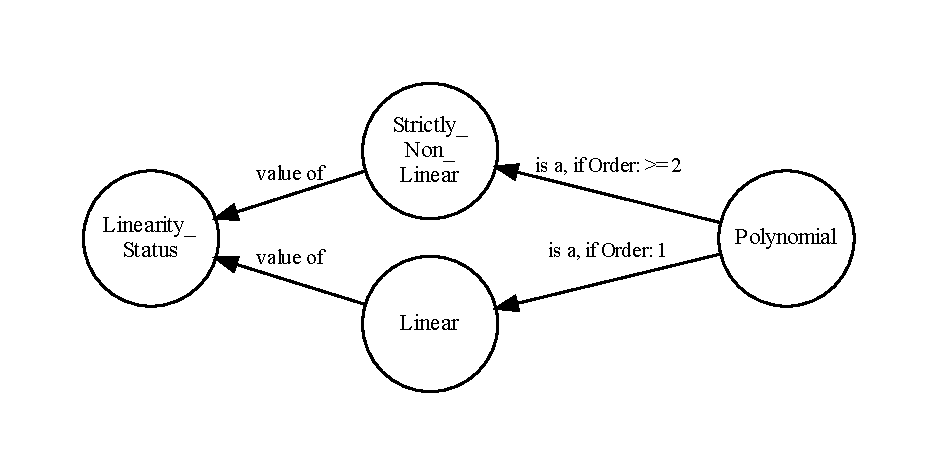
\includegraphics[trim=28 35 28 35, clip, width=0.8\linewidth]{Ausschnitt_KS_Poly_Linearity}} % trim={<left> <lower> <right> <upper>}
		\subcaption{Verworfene Integrationsart für die Kategorie \textit{Polynom} im KS}
	\end{subfigure}
	\begin{subfigure}[c]{0.9\textwidth}
		\centering
		\fbox{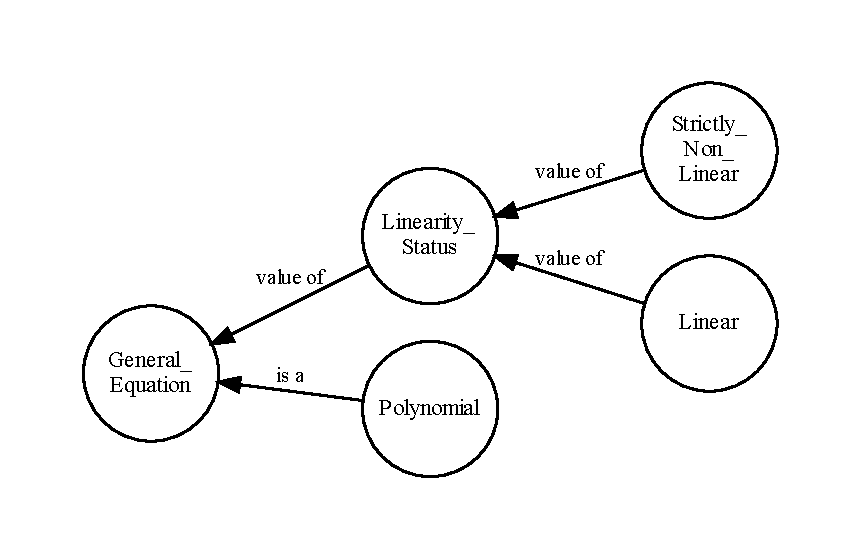
\includegraphics[trim=28 35 28 35, clip, width=0.8\linewidth]{Ausschnitt_KS_Poly_Linearity_Used}}
		\subcaption{Genutzte Integration der Kategorie \textit{Polynom} im KS}
	\end{subfigure}
	\caption{Integrationsmöglichkeiten der Kategorie \textit{Polynom}}
	\label{fig:KS_Poly}
\end{figure}

Problemstellung: \textbf{Polynom}\\
Ein Polynom kann abhängig von seiner Ordnung linear oder nichtlinear sein. Um diesen Sachverhalt vollständig im KS abzubilden müsste das Polynom im KS ein Objekt der Kategorien \textit{Linear} und \textit{Strictly\_Non\_Linear} sein, welche zwei Werte der Kategorie \textit{Linearity} sind, die sich gegenseitig ausschließen. In der Anwendung auf ein Modell lässt sich dieser Widerspruch im Allgemeinen problemlos aufheben, da bei einem spezifischen Modell, dessen Modellgleichungen eine polynomiale Form haben, die Ordnung der Polynome festgelegt ist. Die durch diese Problemstellung aufgetretene Frage ist also: Sollen Widersprüche im KS auftreten dürfen, wenn diese sich bei Anwendung auf ein konkretes Modell aufheben?
\begin{enumerate}[resume*]
	\item \label{E.KS_Widersprüche}Innerhalb KS soll es keine Widersprüche geben.
\end{enumerate}
Der Grund für die Entscheidung ist, dass es in Anbetracht der Anwendbarkeit für sinnvoller erachtet wurde das KS widerspruchsfrei zu gestalten, um das KS intuitiv verständlich zu halten. In Folge dieser Entscheidung wurde das Polynom der Kategorie \textit{Strictly\_Non\_Linear} zugeordnet.












